% This text is proprietary.
% It's a part of presentation made by myself.
% It may not used commercial.
% The noncommercial use such as private and study is free
% Sep. 2005 
% Author: Sascha Frank 
% University Freiburg 
% www.informatik.uni-freiburg.de/~frank/


\documentclass{beamer}
\usepackage{multirow,multicol}
\usepackage{color}
\makeatletter
\newcommand{\redub}{}
\def\redub#1{%
  \@ifnextchar_%
    {\@redub{#1}}
    {\@latex@warning{Missing argument for \string\redub}\@redub{#1}_{}}%
}
\def\@redub #1_#2{%
    \colorlet{currentcolor}{.}%
    \color{red}%
    \underbrace{\color{currentcolor}#1}_{\color{red}#2}%
    \color{currentcolor}%
}
\makeatother

\begin{document}
\title{Stochastic Variational Inference}   
\subtitle{from Hoffman et al., 2013}
\author{Presented By Ryan Cotterell and Frank Ferraro} 
\date{\today} 

\frame{\titlepage} 

%\frame{\frametitle{Table of contents}\tableofcontents} 

\frame{\frametitle{Overview of Variational Inference}
  \begin{itemize}
    \item Turns a complicated inference problems into an optimization problem
    \item Minimizes the KL divergence from the variational distribution to the posterior
      distribution
    \item EM is a special case
  \end{itemize}
}

\frame{\frametitle{Model Image}
put fig 2 here

give gloss of variables: relate them to the input/output/nuissance ones Jason defines
}

\frame{\frametitle{Evidence Lower Bound (ELBO)}
  \begin{itemize}
    \item Key insight is the use of Jensen's inequality
    \item We choose $q$ from some family of distributions $\mathcal{Q}$
  \end{itemize}

  \begin{eqnarray*} %% Do avoid eqnarray if possible.
    \log(p(x \mid \alpha)) & = & \log \int p(x,z,\beta \mid \alpha) dz \ d\beta \\
    \uncover<2->{& = & \log \int p(x,z,\beta \mid \alpha) \frac{q(z,\beta)}{q(z,\beta)} dz d\beta \\}
    \uncover<3->{& = & \log\left(\mathbb{E}_q \left[ \frac{p(x,z,\beta \mid \alpha)}{q(z,\beta)} \right] \right) \\}
    \uncover<4->{& \geq & \mathbb{E}_q \left[ \log p(x,z,\beta \mid \alpha)\right] - \mathbb{E}_q \left[ q(z,\beta) \right] \\}
    \uncover<5->{& = & \mathcal{L}(q)}
  \end{eqnarray*}
}

\frame{\frametitle{Why does maximizes the ELBO minimize the KL-Divergence?} 
  \begin{eqnarray*} %% Do avoid eqnarray if possible.
    \text{KL}(q(z,\beta)||p(z,\beta|x) &=& \mathbb{E}_q \left[ \log(q(z,\beta) \right] - \mathbb{E}_q 
\left[ \log p(z,\beta|x) \right] \\
    & = & \mathbb{E}_q \left[ \log(q(z,\beta) \right] - \mathbb{E}_q 
\left[ \log p(z,\beta,x) \right] + \log p(x) \\
    & = & -\mathcal{L}(q) + const.
    \end{eqnarray*}
    
    \begin{itemize}
      \item Maximizing $\mathcal{L}(q)$ is just minimizing $-\mathcal{L}(q)$
    \end{itemize}

}

\frame{\frametitle{Low Euclidean distance $\neq$ low distribution similarity}
\begin{itemize}
\item $p_1 \sim \mathcal{N}(\mu_1,\sigma_1)$, $p_2 \sim \mathcal{N}(\mu_2,\sigma_2)$
\end{itemize}
\begin{columns}
\begin{column}{.48\textwidth}
%\color{red}\rule{\linewidth}{4pt}
\begin{block}{\small High Euclidean distance, High Distribution similarity}
{\small
$\mu_1=0,\sigma_1=10K$\\
$\mu_2=10,\sigma_2=10K$
}
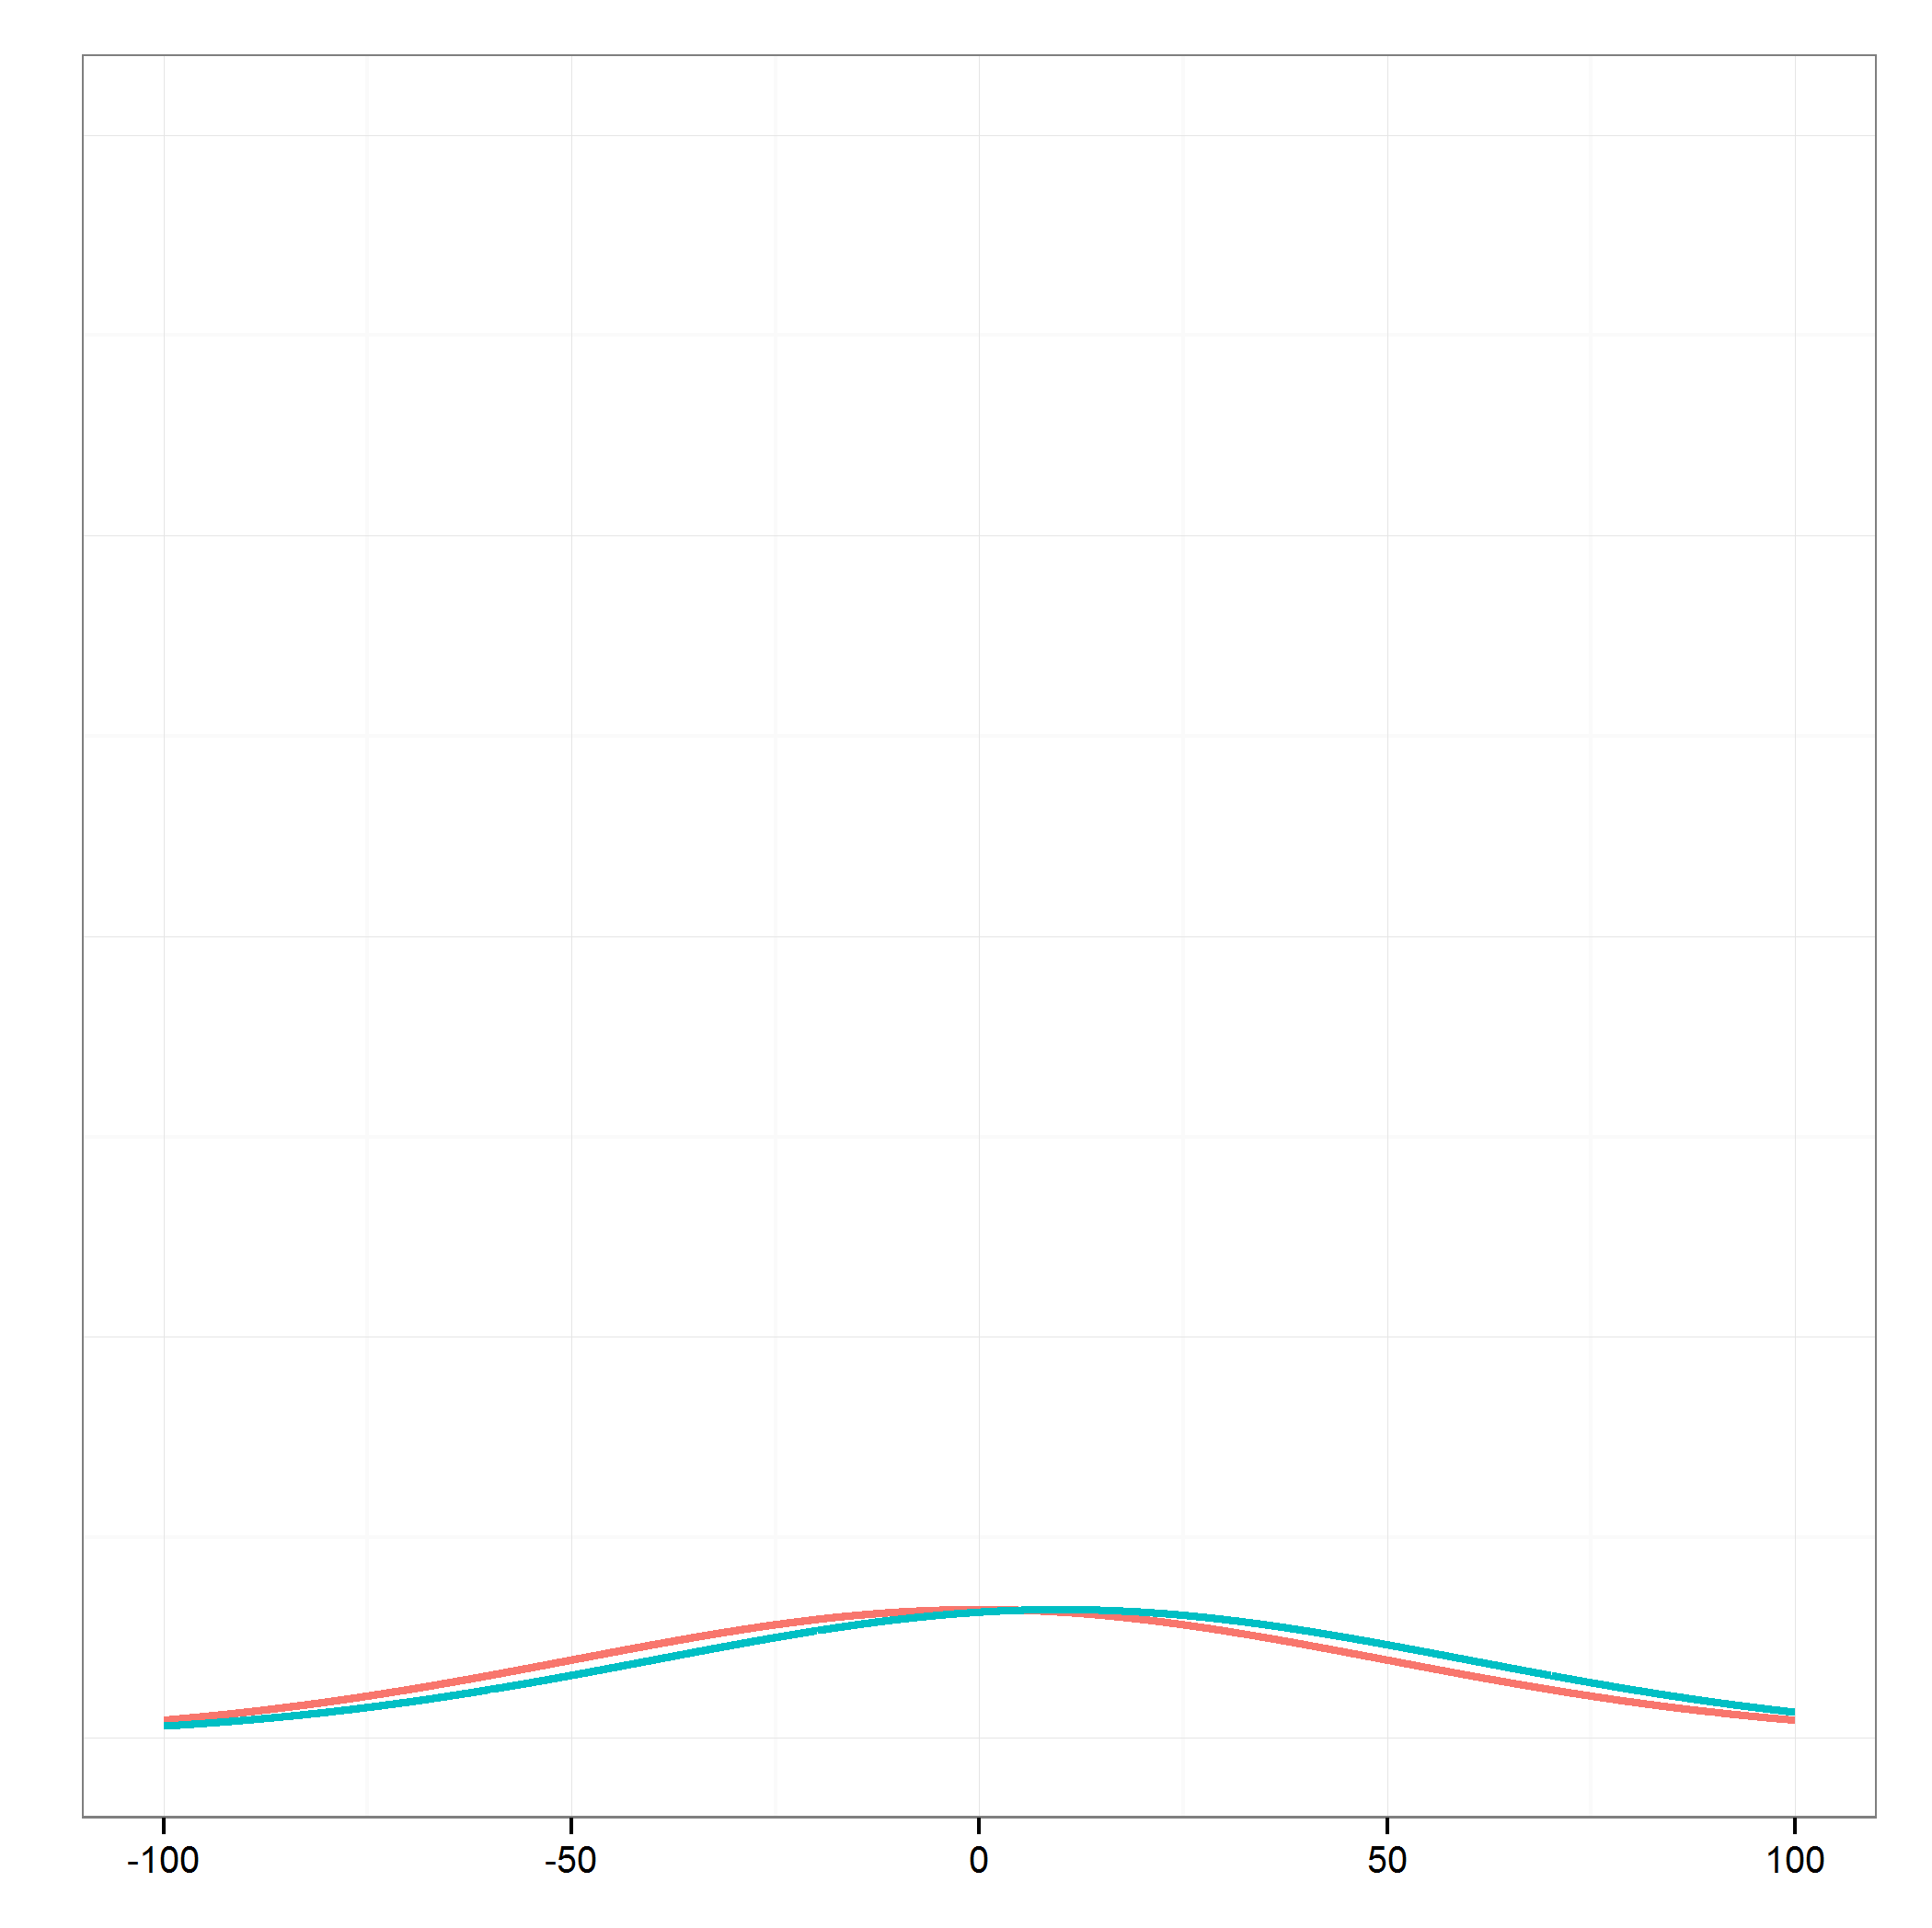
\includegraphics[scale=.3]{figs/first}
\end{block}
\end{column}%
\hfill%
\uncover<2->{
\begin{column}{.48\textwidth}
%\color{blue}\rule{\linewidth}{4pt}
\begin{block}{\small Low Euclidean distance, High Distribution similarity}
{\small
$\mu_1=0,\sigma_1=0.01K$\\
$\mu_2=0.1,\sigma_2=0.01K$
}
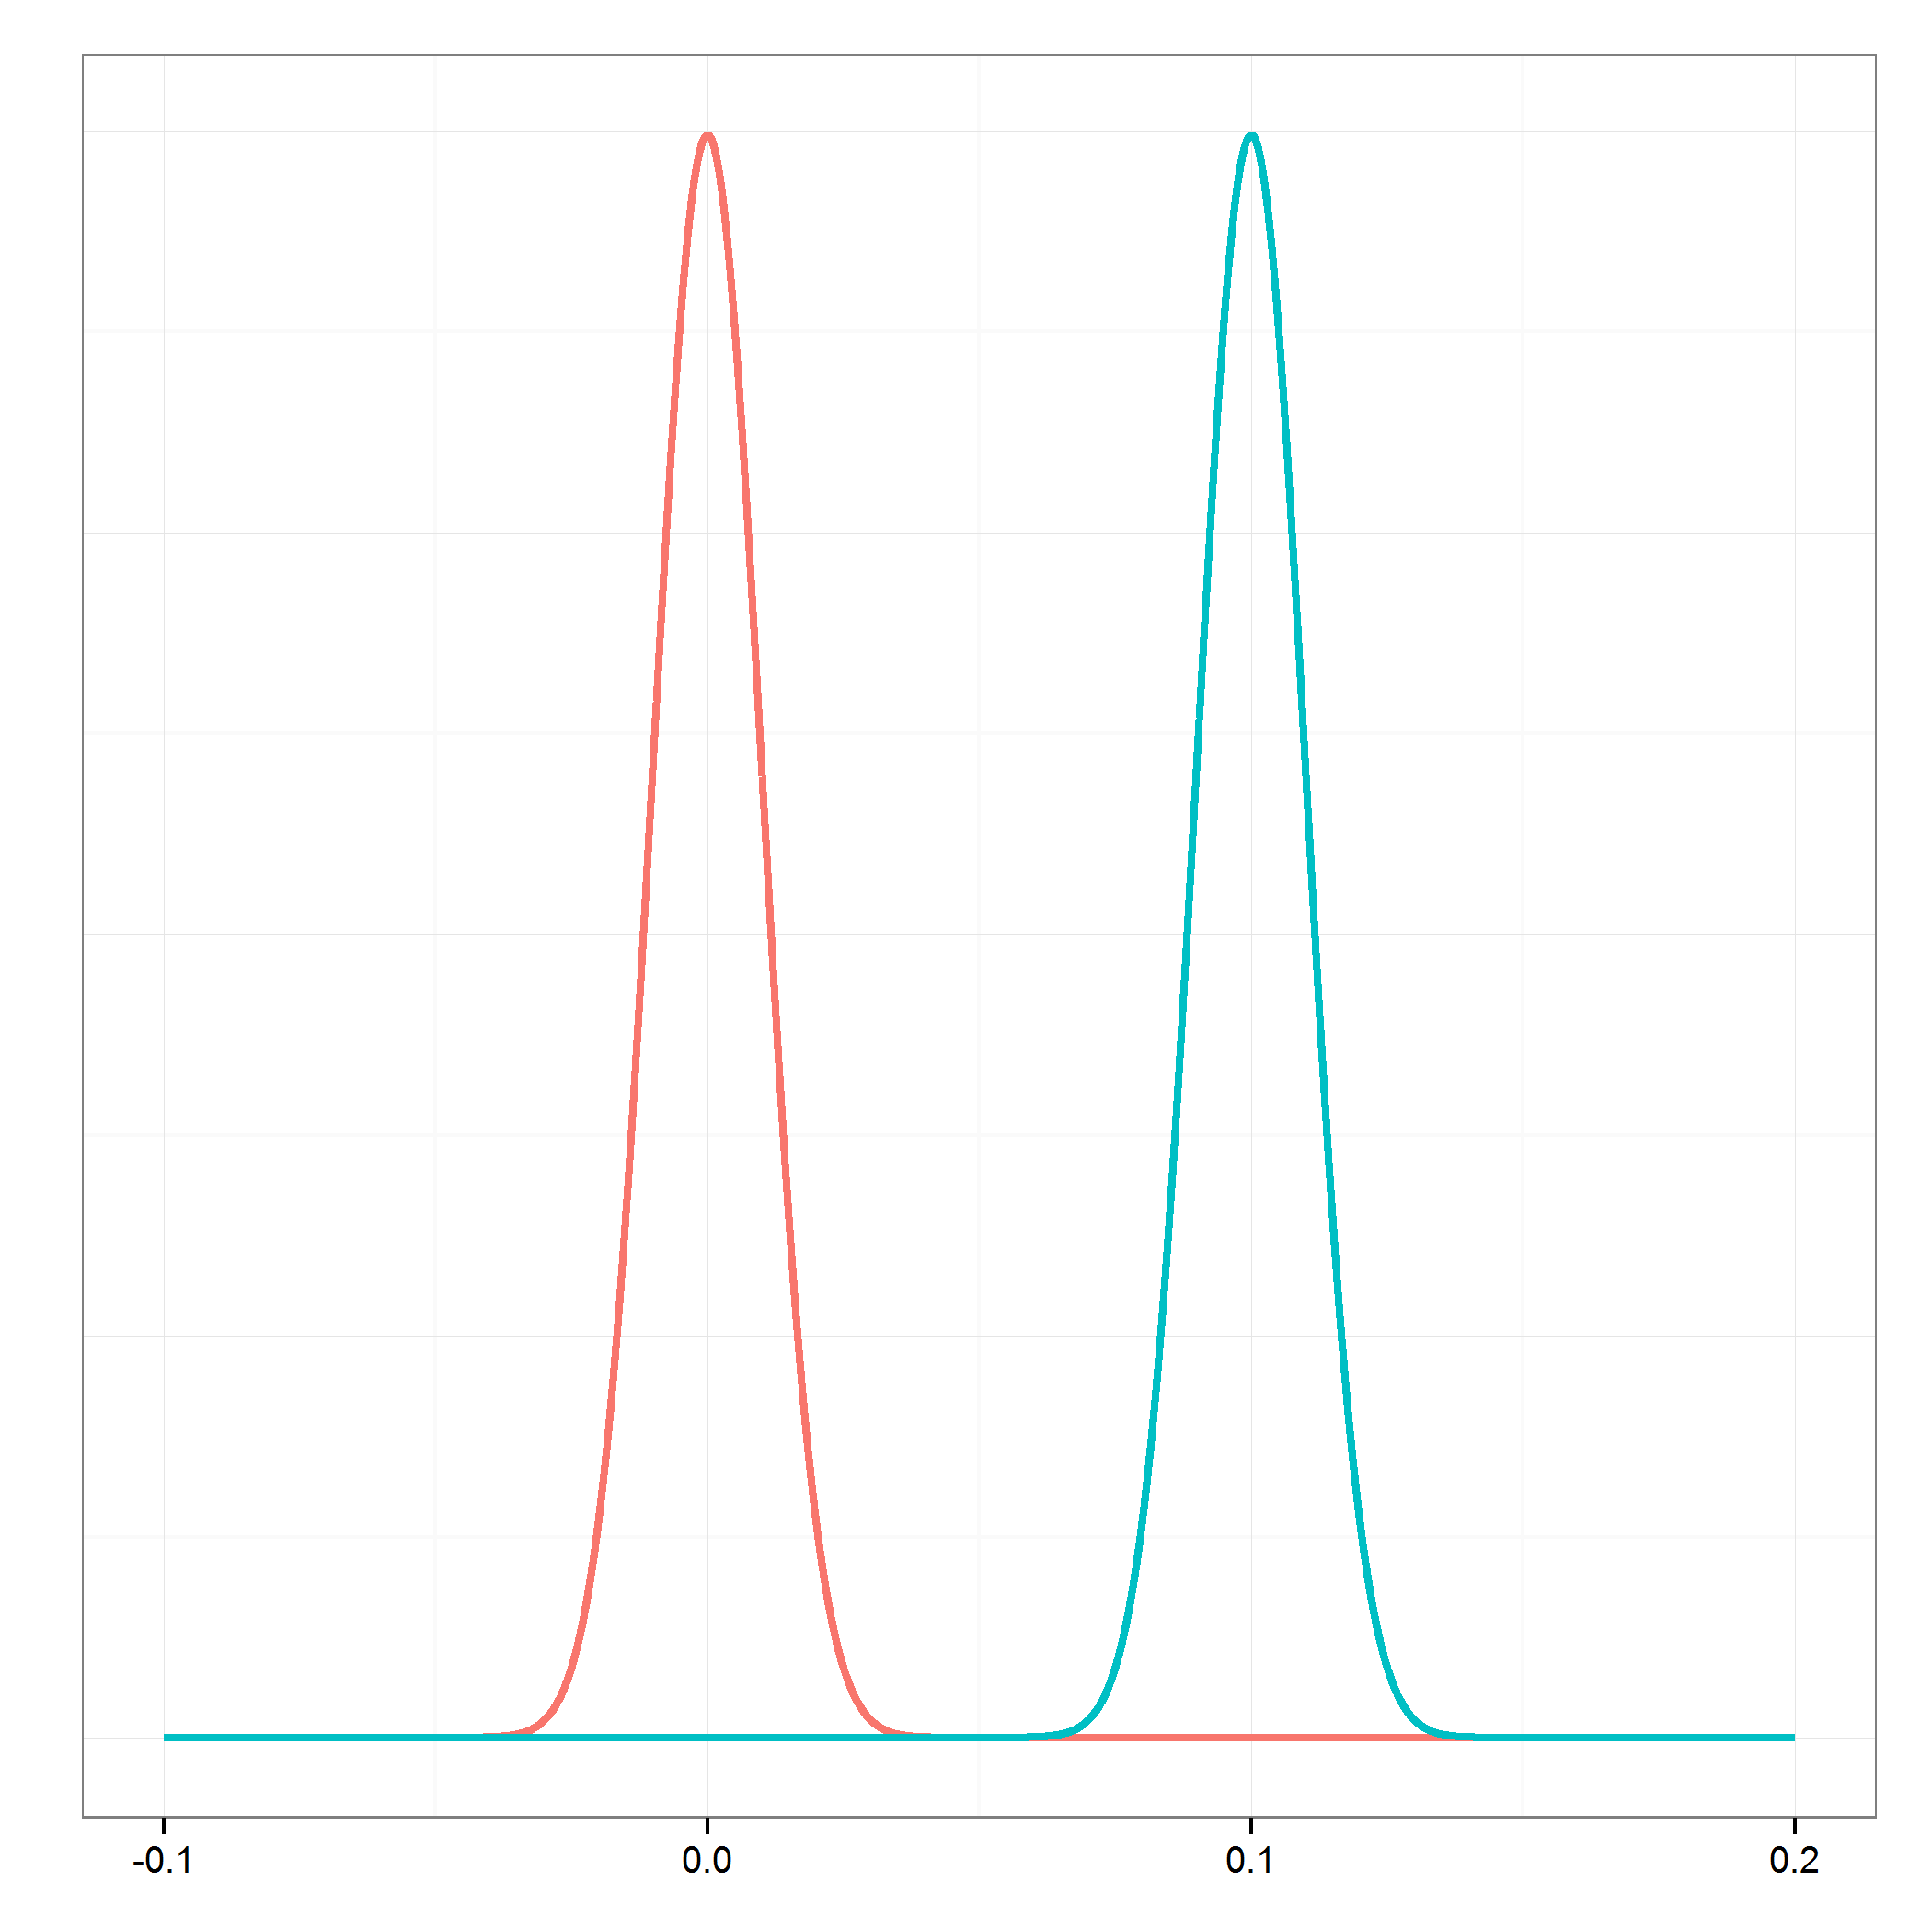
\includegraphics[scale=.3]{figs/second}
\end{block}
\end{column}%
}
\end{columns}
%%%%%%%%%%
}
\frame{\frametitle{Natural Gradient}
 Talk about Natural Gradient
}

\frame{\frametitle{EM vs. Variational Inference}
 Online Variational Inference 4 picture Algorithm Comparison
}

\frame{\frametitle{How is EM a special case?}
  \begin{itemize}
    \item How do we choose $\mathcal{Q}$?
    \item We want it to be easily computable!
    \item What if $p(z,\theta |x) \in \mathcal{Q}$? 
    \item Then computing expectations under $q$ is just inference
      in our model!
    \item Consider a standard HMM, our E-step involves direct computation of the marginals through Forward-Backwards
    \item Let $p_\theta(z|x)$ be our model and $\theta_1$ be a setting of parameters
      where $z$ is a latent variable (tags in an HMM) and $x$ is an observed variable (words in an HMM)
    \item Since $p_\theta \in \mathcal{Q},\; \forall \theta \in \Theta$, we simply need to maximize
      $\sum_z p(z|x;\theta_1) \log\left(p(z|x; \theta_2)\right)$ with respect to $\theta_2$
  \end{itemize}
  

}
 

\frame{\frametitle{Variational + $x,\; \forall x$}
  \begin{itemize}
    \item Variational EM - the process described above
    \item Variational Bayes - approximate inference (no M-step)
    \item Variational Decoding - approximation decoding 
      
  \end{itemize}

}


%\section{Section no. 2} 
%\subsection{Lists I}
%\frame{\frametitle{unnumbered lists}
%\begin{itemize}
%\item Introduction to  \LaTeX  
%\item Course 2 
%\item Termpapers and presentations with \LaTeX 
%\item Beamer class
%\end{itemize} 
%}
%
%\frame{\frametitle{lists with pause}
%\begin{itemize}
%\item Introduction to  \LaTeX \pause 
%\item Course 2 \pause 
%\item Termpapers and presentations with \LaTeX \pause 
%\item Beamer class
%\end{itemize} 
%}
%
%\subsection{Lists II}
%\frame{\frametitle{numbered lists}
%\begin{enumerate}
%\item Introduction to  \LaTeX  
%\item Course 2 
%\item Termpapers and presentations with \LaTeX 
%\item Beamer class
%\end{enumerate}
%}
%\frame{\frametitle{numbered lists with pause}
%\begin{enumerate}
%\item Introduction to  \LaTeX \pause 
%\item Course 2 \pause 
%\item Termpapers and presentations with \LaTeX \pause 
%\item Beamer class
%\end{enumerate}
%}
%
%\section{Section no.3} 
%\subsection{Tables}
%\frame{\frametitle{Tables}
%\begin{tabular}{|c|c|c|}
%\hline
%\textbf{Date} & \textbf{Instructor} & \textbf{Title} \\
%\hline
%WS 04/05 & Sascha Frank & First steps with  \LaTeX  \\
%\hline
%SS 05 & Sascha Frank & \LaTeX \ Course serial \\
%\hline
%\end{tabular}}
%
%
%\frame{\frametitle{Tables with pause}
%\begin{tabular}{c c c}
%A & B & C \\ 
%\pause 
%1 & 2 & 3 \\  
%\pause 
%A & B & C \\ 
%\end{tabular} }
%
%
%\section{Section no. 4}
%\subsection{blocs}
%\frame{\frametitle{blocs}
%
%\begin{block}{title of the bloc}
%bloc text
%\end{block}
%
%\begin{exampleblock}{title of the bloc}
%bloc text
%\end{exampleblock}
%
%
%\begin{alertblock}{title of the bloc}
%bloc text
%\end{alertblock}
%}
\end{document}

